\documentclass{CompilerAssignment}
\usepackage{multirow}
\usepackage{extarrows}
\usepackage{subfig}
\usepackage{tikz}
\usepackage[scheme=plain]{ctex}
\usepackage{newtxtext}

\newcommand{\lmd}{\xLongrightarrow[lm]{}}
\newcommand{\rmd}{\xLongrightarrow[rm]{}}
\renewcommand{\lmd}{\underset{lm}{\Rightarrow}}
\renewcommand{\rmd}{\underset{rm}{\Rightarrow}}
\newcommand{\rma}{\mathrm{a}}
\newcommand{\first}{\text{FIRST}}
\newcommand{\follow}{\text{FOLLOW}}

\title{Assignment 3}

\begin{document}

\maketitle

\section{Required Exercises}

\subsection{Exercise 1}

% \begin{equation}
%     S \rightarrow SS+ \ |\ SS* \ |\ \rma
% \end{equation}

\begin{enumerate}
    \item No, it isn't.
    \item \(S \lmd SS* \lmd SS*S* \lmd \rma S*S* \lmd \rma\rma *S* \lmd \rma\rma *SS+* \lmd \rma\rma *\rma S+* \lmd \rma\rma *\rma\rma +*\).
    \item \(S \rmd SS* \rmd SSS+* \rmd SS\rma+* \rmd S\rma\rma+* \rmd SS*\rma\rma+* \rmd S\rma *\rma\rma+* \rmd \rma\rma *\rma\rma+*\).
    \item The parse tree is depicted as follows.
    \begin{center}
        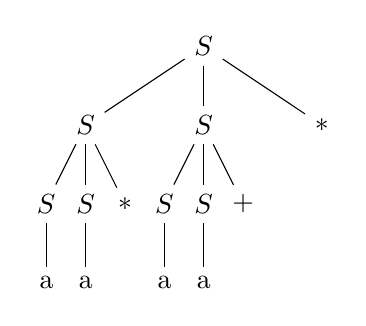
\begin{tikzpicture}
            \node(1) at (0, 0) {\(S\)};
            \node(2) at (-1.5, -1) {\(S\)};
            \node(3) at (0, -1) {\(S\)};
            \node(4) at (1.5, -1) {\(*\)};
            \path[] (1) edge (2) (1) edge (3) (1) edge (4);
            \node(5) at (-2, -2) {\(S\)};
            \node(6) at (-1.5, -2) {\(S\)};
            \node(7) at (-1, -2) {\(*\)};
            \path[] (2) edge (5) (2) edge (6) (2) edge (7);
            \node(8) at (-0.5, -2) {\(S\)};
            \node(9) at (0, -2) {\(S\)};
            \node(10) at (0.5, -2) {\(+\)};
            \path[] (3) edge (8) (3) edge (9) (3) edge (10);
            \node(11) at (-2, -3) {a};
            \node(12) at (-1.5, -3) {a};
            \node(13) at (-0.5, -3) {a};
            \node(14) at (0, -3) {a};
            \path[] (5) edge (11) (6) edge (12) (8) edge (13) (9) edge (14);
        \end{tikzpicture}
    \end{center}
    \item The grammar can be rewritten as follows.
    \begin{equation*}
        \begin{aligned}
            S \rightarrow\ & \rma S', \\
            S' \rightarrow\ & S + S' \ |\ S * S' \ |\ \epsilon.
        \end{aligned}
    \end{equation*}
\end{enumerate}

\subsection{Exercise 2}

% \begin{equation}
%     \begin{aligned}
%         S \rightarrow\ & \rma B, \\
%         B \rightarrow\ & S + B \ |\ \epsilon.
%     \end{aligned}
% \end{equation}

\begin{enumerate}
    \item
    \begin{enumerate}
        \item Calculate the FIRST and FOLLOW sets for the grammar.
        \begin{align*}
            \first(S) &= \{ \rma \}, \\
            \first(B) &= \first(S) \cup \{ \epsilon \} = \{ \rma, \epsilon \}, \\
            \follow(S) &= \{ +, \$ \}, \\
            \follow(B) &= \follow(S) \cup \{\$\} = \{ +, \$ \}.
        \end{align*}
        \item Construct the predictive parsing table for the grammar.
        \begin{center}
            \begin{tabular}{c|ccc}
                \hline \hline
                \multirow{2}{*}{\textsc{Non-Terminal}} & \multicolumn{3}{c}{\textsc{Input Symbol}} \\
                                  & a     & $+$    & \$    \\
                \hline
                $S$               & $S \rightarrow \rma B$ &      &       \\
                $B$               & $B \rightarrow S + B$ & $B \rightarrow \epsilon$ & $B \rightarrow \epsilon$ \\ \hline
            \end{tabular}
        \end{center}
    \end{enumerate}
    \item Yes, it is.
    \item Yes, it can. The moves are listed as follows.
    \begin{center}
        \begin{tabular}{lrrl}
            \hline \hline
            \textsc{Matched} & \textsc{Stack} & \textsc{Input} & \textsc{Action} \\ \hline
            & $S\$$ & aaaa$+++$\$ & \\
            & $\rma B\$$ & aaaa$+++$\$ & output $S \rightarrow \rma B$ \\
            a & $B\$$ & aaa$+++$\$ & match a \\
            a & $S + B\$$ & aaa$+++$\$ & output $B \rightarrow S + B$ \\
            a & $\rma B + B\$$ & aaa$+++$\$ & output $S \rightarrow \rma B$ \\
            aa & $B + B\$$ & aa$+++$\$ & match a \\
            aa & $S + B + B\$$ & aa$+++$\$ & output $B \rightarrow S + B$ \\
            aa & $\rma B + B + B\$$ & aa$+++$\$ & output $S \rightarrow \rma B$ \\
            aaa & $B + B + B\$$ & a$+++$\$ & match a \\
            aaa & $S + B + B + B\$$ & a$+++$\$ & output $B \rightarrow S + B$ \\
            aaa & $\rma B + B + B + B\$$ & a$+++$\$ & output $S \rightarrow \rma B$ \\
            aaaa & $B + B + B + B\$$ & $+++$\$ & match a \\
            aaaa & $+ B + B + B\$$ & $+++$\$ & output $B \rightarrow \epsilon$ \\
            aaaa$+$ & $B + B + B\$$ & $++$\$ & match + \\
            aaaa$+$ & $+ B + B\$$ & $++$\$ & output $B \rightarrow \epsilon$ \\
            aaaa$++$ & $B + B\$$ & $+$\$ & match + \\
            aaaa$++$ & $+ B\$$ & $+$\$ & output $B \rightarrow \epsilon$ \\
            aaaa$+++$ & $B\$$ & \$ & match + \\
            aaaa$+++$ & $\$$ & \$ & output $B \rightarrow \epsilon$ \\ \hline
        \end{tabular}
    \end{center}
\end{enumerate}

\section{Optional Exercises}

\subsection{Exercise 1}

Yes, it is ambiguous.

e.g. 我喜欢你讨厌他

\begin{figure}[!h]
    \centering
    \subfloat[Parse tree 1]{
        \begin{tikzpicture}
            \node(1) at (-1, 0) {短语};
            \node(2) at (-3, -1) {短语};
            \node(3) at (-1, -1) {动词};
            \node(4) at (1, -1) {短语};
            \path[] (1) edge (2) (1) edge (3) (1) edge (4);
            \node(5) at (-4, -2) {短语};
            \node(6) at (-3, -2) {动词};
            \node(7) at (-2, -2) {短语};
            \path[] (2) edge (5) (2) edge (6) (2) edge (7);
            \node(8) at (-4, -3) {人};
            \node(9) at (-3, -3) {喜欢};
            \node(10) at (-2, -3) {人};
            \path[] (5) edge (8) (6) edge (9) (7) edge (10);
            \node(11) at (-1, -2) {讨厌};
            \node(12) at (1, -2) {人};
            \path[] (3) edge (11) (4) edge (12);
            \node(13) at (-4, -4) {我};
            \node(14) at (-2, -4) {你};
            \node(15) at (1, -3) {他};
            \path[] (8) edge (13) (10) edge (14) (12) edge (15);
        \end{tikzpicture}
    }\qquad\qquad
    \subfloat[Parse tree 2]{
        \begin{tikzpicture}
            \node(1) at (-1, 0) {短语};
            \node(2) at (-3, -1) {短语};
            \node(3) at (-1, -1) {动词};
            \node(4) at (1, -1) {短语};
            \path[] (1) edge (2) (1) edge (3) (1) edge (4);
            \node(5) at (0, -2) {短语};
            \node(6) at (1, -2) {动词};
            \node(7) at (2, -2) {短语};
            \path[] (4) edge (5) (4) edge (6) (4) edge (7);
            \node(8) at (0, -3) {人};
            \node(9) at (1, -3) {讨厌};
            \node(10) at (2, -3) {人};
            \path[] (5) edge (8) (6) edge (9) (7) edge (10);
            \node(11) at (-3, -2) {人};
            \node(12) at (-1, -2) {喜欢};
            \path[] (2) edge (11) (3) edge (12);
            \node(13) at (0, -4) {你};
            \node(14) at (2, -4) {他};
            \node(15) at (-3, -3) {我};
            \path[] (8) edge (13) (10) edge (14) (11) edge (15);
        \end{tikzpicture}
    }
    \caption{Two parse trees for the ambiguous sentence}
\end{figure}

\end{document}